%%%%%%%%%%%%%%%%%%%%%%%%%%%%%%%%%%%%%%%%%%%%%%%%%%%%
\section{The BDI Learning Framework}\label{sec:framework}
%%%%%%%%%%%%%%%%%%%%%%%%%%%%%%%%%%%%%%%%%%%%%%%%%%%%

Our learning task may be summarised as follows: \textit{Given past execution data and the current world state, determine which plan to execute next in order to best address the event-goal in question}. In the BDI sense, our task is to learn the context condition of each plan in the goal-plan hierarchy. In this section we describe our BDI Learning Framework that enables such learning. In particular we describe the use of \dt s for learning context conditions, together with the confidence-based probabilistic plan selection that uses the learning output, with a focus on learning with event-goal types and recursive event-goals.

\subsection{Integrating Decision Trees into Context Conditions for Plans}\label{sec:introlearning}

In a BDI system, a plans context condition is a logical formula that is constructed at design time and evaluated against an event-goal at run time to determine if the plan is applicable in the given world state\footnote{Context formulas may reference internal beliefs as well as environment states, and for this study we treat both as inclusive in the world state.}. As reported in \cite{Airiau:IJAT:09}, in order to allow the context condition to be learnt over time, we annotate each plans context formula with a \textit{\dt}\footnote{It is perfectly feasible to combine the existing logical formula with the \dt\ classification, but to aid our understanding of the \dt\ learning in this study we always use an empty initial formula.}. The idea is that the agent starts with some \textit{necessary but possibly insufficient} conditions for each plan (provided by the designer), and over time and in the course of trying various plans in various world states will be able to \textit{refine} each plans context condition using the learnt \dt\ classification of the world states encountered.

The choice of \dt s as the learning module is motivated by several factors. Firstly, \dt s support hypotheses that are a disjunction of conjunctive terms, and since context formulas are generally expressed in this form then \dt s are readily applicable. Secondly, \dt s can be converted to \textit{if-then} rules that are human readable and can therefore be verified by a domain expert. Finally, \dt s are robust against training data that may contain errors. This is specially relevant in a stochastic domain where perfectly applicable plans may nevertheless fail due to unforeseen circumstances.

The input for the \dt\ learning is a training set of data points of the form $[w,o]$, where $w$ is the world state in which the plan was executed and $o$ was the boolean outcome (success or failure). Initially the training set is empty and grows over time as the agent tries the plan in various world states and samples the result. The world state $w$ itself is a set of discrete attributes that together represent the state of affairs. The idea is that over time the \dt\ will learn a classification based purely on the subset of attributes in $w$ that are relevant to the context condition of the plan. 

The attributes in $w$ determine the quality of the final classification, and their number and possible values has a bearing on the size of the training set required to correctly learn the context condition. The choice of attributes to include in the world state $w$ is a design decision and dependent on domain knowledge. Importantly, the attributes in $w$ should be a superset of the necessary and sufficient attributes relevant to the context condition. For instance, for a plan to pick up an object using a robotic arm, \textit{objectSurface} is a relevant attribute, \textit{gripperWet} possibly is, but \textit{dayOfWeek} likely is not. For the purpose of our study we assume that the designer provides a set of all attributes that are considered possibly relevant to the context condition of the plan. In the worst case, this set is the full set of attributes of the world. 

The decision tree inductive bias is a preference for smaller trees. In other words, the induction of \dt s will trade-off some accuracy in classification for compactness of representation. In fact such inductive bias is necessary if the \dt\ is to generalise to as yet unseen world states. Once a \dt\ is induced from the training set, it may be used to classify any new world state $w$. In the strict sense the classification is an outcome $o$ (failure or success). However, several \dt\ implementations including \propername{J48} in \weka\footnote{In our study we use algorithm \propername{J48}, a version of \propername{c4.5} \cite{Mitchell97:ML}, from the \weka\ learning package \cite{weka99}.} annotate a likelihood of class membership (that is indicative of the inductive bias) to the returned classification. For the given world state $w$ then, we treat the returned likelihood of membership to the $success$ class as the expected likelihood of success of the plan.

One source of misclassification in the learnt \dt s is from erroneous training samples collected when a plan fails not because it was a bad choice in the given world state, but because a bad choice was made somewhere in the execution path below it in the BDI goal-plan hierarchy. Previously in \cite{Airiau:IJAT:09} we have shown how \textit{selective recording} of outcomes may be used to overcome this issue.

A second source of misclassification is from the unorthodox use of \dt s in our framework. Note that the typical use of \dt s lies in the \textit{offline} induction from a complete training set. However, in our case training samples are progressively added after each new execution, while all the time the agent makes the best choice given the experience so far. This results in an incomplete training set in the early stages of learning\footnote{Training data is incomplete in the sense that the agent has only collected a portion of the full data set required to learn the correct classification.} leading to misclassification errors. In \cite{Singh:AAMAS10} we show how a measure of confidence in the \dt\ classification based on the \textit{coverage} of the paths \textit{below} the plan in the goal-plan hierarchy may be used \textit{during plan selection} to address this issue (independent of the recording scheme used).


\subsection{Confidence-based Probabilistic Plan Selection}

In previous work \cite{Singh:AAMAS10} we introduced a confidence measure in the \dt\ classification based on the notion of \textit{coverage} of the choices below the plan in the BDI goal-plan hierarchy. The idea is that our confidence in a plan's \dt\ increases as more of the possible execution paths below the plan in the goal-plan hierarchy are explored.

\begin{equation*}\label{eqn:coverage}   
\Omega_P(w) = 0.5 + \left[  c_P(w) *  \left( \kappa_P(w) - 0.5 \right)  \right].
\end{equation*}

Equation \ref{eqn:coverage} shows how the final plan selection weight $\Omega'_T(w)$ is calculated for a given world state $w$. Initially, the selection weight for a previously unseen world state $w$ takes the default value of $0.5$. Over time, as the various execution paths below the plan are tried in $w$, its coverage $c_P(w)$ increases and the selection weight approaches the value $\kappa_P(w)$ estimated by the plan's \dt.

The \emph{probabilistic plan selection} scheme states that, given an event-goal
$e$ to be resolved in a world/belief state $w$, the agent chooses a plan $P_i$
among the relevant plans for $e$ with a probability directly proportional to its
estimation of success in state $w$ (by $P_i$'s decision tree) and normalized
among all the success estimation of all relevant options. An default success
estimation of $.5$ is used for plans that have never been executed.
% %
Using such a probabilistic plan selection, the BDI learning system allows for both
\emph{exploitation} and \emph{exploration} of the given know-how information
encoded in the plan library.
% %
Observe that typical BDI platforms do offer various advanced mechanisms for plan
selection, including plan precedence and meta-level reasoning. However, these
mechanisms are pre-programmed and do not take into account the experience of the
agent.



\subsection{Handling Event-Goal Types}
Recall our previous definition of the learning task: \textit{Given past execution data and the current world state, determine which plan to execute next in order to best address the event-goal in question}. The simplifying assumption in this definition is that the event-goal in question is an \textit{event-goal instance}. In practical BDI systems, it is often the case that a single plan will handle all instances of an \textit{event-goal type}. Furthermore event-goal instance parameters will generally be included in the context logical formula. Our BDI learning framework account presented earlier in \cite{Airiau:IJAT:09} and \cite{Singh:AAMAS10} did not address the issue of learning context conditions for plans that handle event-goal types, and is the subject of this study.

For the purpose of learning context conditions, we treat the event-goal parameters as relevant attributes of the world. As such, the training set then contains samples of the form $[w \cup \varphi,o]$ where the world state $w$ is the initial set of all relevant attributes that represent the state of affairs, $\varphi$ is the set of all event-type parameters, and $o$ is the outcome class (success or failure). This way, incorporating $\varphi$ in the training data is the only step required for handling event-goal types and no change to the actual framework is warranted.

\subsection{Support for Recursive Event-Goals}

Recursion in the context of event-goals refers to the case where the resolution of an event-goal instance $G[\varphi_1]$ involves first the resolution of another goal-event instance $G[\varphi_2]$ of the same type. The result is a growing stack of pending $G[\varphi_i]$ event-goals that eventually terminate in $G[\varphi_n]$ whose parameters satisfy the termination conditions i.e. where a non-recursive plan choice is made.

In order to better understand the impact of recursion on context learning, we use the notion of an \textit{execution trace} that is a sequence of the form $G_0\langle\varphi_0\rangle[P_0:w_0] \cdot G_1\langle\varphi_1\rangle[P_1:w_1] \cdot \ldots \cdot G_n\langle\varphi_1\rangle[P_n:w_n]$, that represents a sequence of event-goals along with the plans selected to handle them and the world state in which the selections were made. So $G_i\langle\varphi_i\rangle[P_i:w_i]$ captures the case where plan $P_i$ was selected in world state $w_i$ in order to achieve the goal-event $G_i\langle\varphi_i\rangle$.

\begin{figure}[t]
\begin{center}
\resizebox{0.8\textwidth}{!}{
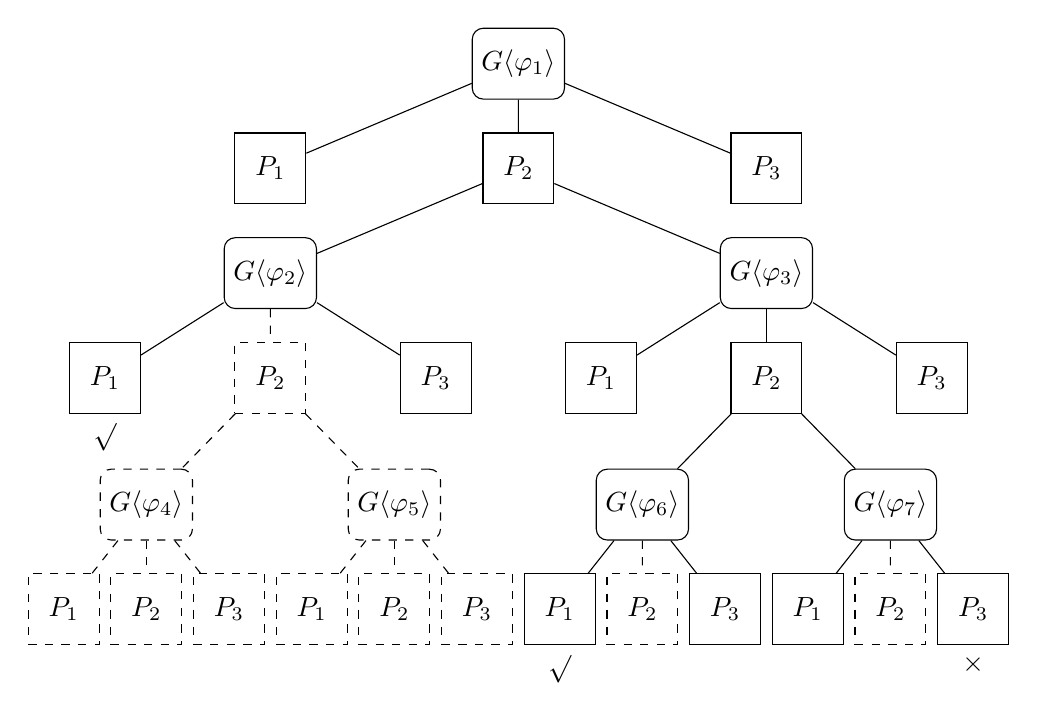
\begin{tikzpicture}[scale=0.7]
\tikzstyle{txt}=[scale=1.0]
\tikzstyle{succ}=[label=below:$\surd$]
\tikzstyle{fail}=[label=below:$\times$]
\tikzstyle{planbox}=[draw,minimum height=0.9cm,minimum width=0.9cm]
\tikzstyle{goalbox}=[draw,rounded corners,minimum height=0.9cm,minimum width=1.0cm]
\tikzstyle{level 1}=[sibling distance=4.5cm,level distance=1.9cm] 
\tikzstyle{level 2}=[sibling distance=9.0cm,level distance=1.9cm] 
\tikzstyle{level 3}=[sibling distance=3.0cm,level distance=1.9cm]
\tikzstyle{level 4}=[sibling distance=4.5cm,level distance=2.3cm]
\tikzstyle{level 5}=[sibling distance=1.5cm,level distance=1.9cm]
\tikzstyle{level 6}=[sibling distance=1.3cm,level distance=1.9cm]

\node[goalbox,yshift=1cm] {$G\langle\varphi_1\rangle$}
	child {node[planbox] {$P_1$}}
	child {node[planbox] {$P_2$}
		child {node[goalbox] {$G\langle\varphi_2\rangle$}
			child {node[planbox,succ] {$P_1$}}
			child[dashed] {node[planbox] {$P_2$}
				child {node[goalbox] {$G\langle\varphi_4\rangle$}
					child {node[planbox] {$P_1$}}
					child {node[planbox] {$P_2$}}
					child {node[planbox] {$P_3$}}
				}
				child {node[goalbox] {$G\langle\varphi_5\rangle$}
					child {node[planbox] {$P_1$}}
					child {node[planbox] {$P_2$}}
					child {node[planbox] {$P_3$}}
				}
			}
			child {node[planbox] {$P_3$}}
		}
		child {node[goalbox] {$G\langle\varphi_3\rangle$}
			child {node[planbox] {$P_1$}}
			child {node[planbox] {$P_2$}
				child {node[goalbox] {$G\langle\varphi_6\rangle$}
					child {node[planbox,succ] {$P_1$}}
					child[dashed] {node[planbox] {$P_2$}}
					child {node[planbox] {$P_3$}}
				}
				child {node[goalbox] {$G\langle\varphi_7\rangle$}
					child {node[planbox] {$P_1$}}
					child[dashed] {node[planbox] {$P_2$}}
					child {node[planbox,fail] {$P_3$}}
				}
			}
			child {node[planbox] {$P_3$}}
		}
	}
	child {node[planbox] {$P_3$}}
;

\end{tikzpicture}

}
\end{center}
\caption{Goal-plan hierarchy $\T_2$ containing a single goal type $G\langle\rangle$ handled by three plans $P_1$, $P_2$ and $P_3$. Here plan $P_2$ posts two instances of $G\langle\rangle$ resulting in recursion. Two levels of recursive unfolding are shown. Dashed $P_2$ nodes indicate roots of unexplored recursive sub-trees.}
\label{fig:unfolding}
\end{figure}

Consider the example BDI goal-plan hierarchy $\T_2$ of Figure \ref{fig:unfolding}. The structure has just a single event-goal type $G\langle\rangle$ and three options to handle it, one of which ($P_2$) in turn posts two instances of the same event-goal type $G\langle\rangle$. In this way, the only plans that take an action in the environment are $P_1$ and $P_3$. The figure highlights an execution trace as follows: \[
\lambda=G\langle\varphi_1\rangle[P_2:w_1] \cdot G\langle\varphi_2\rangle[P_1:w_1] \cdot G\langle\varphi_3\rangle[P_2:w_2] \cdot G\langle\varphi_6\rangle[P_1:w_2] \cdot G\langle\varphi_7\rangle[P_3:w_3].
\]

Here, the first choice is the selection of plan $P_2$ to handle event-goal instance $G\langle\varphi_1\rangle$ in a given world $w_1$. Plan $P_2$ in turn immediately posts the event-goal instance $G\langle\varphi_2\rangle$ that is successfully handled by the non-recursive node $P_1$. Plan $P_2$ then posts the second event-goal instance $G\langle\varphi_3\rangle$, which then is handled by itself in a recursive manner.  event-goal $G\langle\varphi_7\rangle$
$\lambda$ traces a path that involves the successive execution of leaf plan $P_1$ for event-goal $G\langle\varphi_2\rangle$ followed by another execution of $P_1$ this time for event-goal $G\langle\varphi_6\rangle$, and finally terminates in the failure of leaf plan $P_3$ for event-goal $G\langle\varphi_7\rangle$. If plan $P_2$ had instead been selected to handle $G\langle\varphi_7\rangle$ then a deeper recursive call would have ensued. Similarly if earlier in the execution trace plan $P_2$ was selected to handle event-goal $G\langle\varphi_2\rangle$ then a different recursive sub-tree (shown in Figure \ref{fig:unfolding} as dotted nodes under $G\langle\varphi_2\rangle$) would have unfolded.

The immediate implication of a recursive goal-plan structure is that the size of the hierarchy is no longer static but instead unfolds in a dynamic manner. The issue stems from the fact that the recursion is \textit{unbounded} because the context conditions that cause the recursion to terminate are initially unknown. So in order to know the context conditions we must recursively explore, but in doing so we risk an infinite recursive call because the context conditions that ought to guide the recursive exploration towards termination are unknown. This means that we may never find the ``bottom'' or leaf nodes. This has implications for any \textit{bottom-up} strategies. For instance, our conservative recording approach of \cite{Airiau:IJAT:09} and the coverage-based confidence measure of \cite{Singh:AAMAS10} both suffer from this problem. Interestingly, the simpler aggressive recording approach is not impacted by recursion as it does not consider the goal-plan structure . 

We now focus on how the coverage-based confidence measure of \cite{Singh:AAMAS10} may be extended for use in recursive hierarchies.


%Explain the compounding during recursive unfolding. Unfolding structure diagram

%Simplifications: Only single level goal recursion allowed ie G1->P1->G1 and not  G1->P1->G2->P2->G. Also no information of Gs in the system so only the parent goal recursion is tracked.

%\subsubsection{Discussion}
%Can we calculate $c_P(w,r)$ for any r if we have witnessed one r? 
